\documentclass[letterpaper,14pt,titlepage,fleqn]{article}

\setlength{\mathindent}{1cm}

\usepackage{graphicx}                                        

\usepackage{amssymb}                                         
\usepackage{amsmath}                                         
\usepackage{amsthm}                                          

\usepackage{alltt}                                           
\usepackage{float}
\usepackage{color}

\usepackage{url}

\usepackage{balance}
\usepackage[TABBOTCAP, tight]{subfigure}
\usepackage{enumitem}

\usepackage{pstricks, pst-node}

\usepackage{cite}
\usepackage{indentfirst}
\usepackage{listings}

% the following sets the geometry of the page
\usepackage{geometry}
\geometry{textheight=9in, textwidth=6.5in}

% random comment

\newcommand{\cred}[1]{{\color{red}#1}}
\newcommand{\cblue}[1]{{\color{blue}#1}}

\usepackage{hyperref}

\usepackage{textcomp}
\usepackage{listings}

\def\name{Haoxiang Wang; Student ID: 932359049}

%% The following metadata will show up in the PDF properties
\hypersetup{
  colorlinks = true,
  urlcolor = black,
  pdfauthor = {\name},
  pdfkeywords = {CS557 Project 1},
  pdftitle = {Project \#2: Noisy Displaced Elliptical Dots},
  pdfsubject = {Project \#2: Noisy Displaced Elliptical Dots},
  pdfpagemode = UseNone
}

\parindent = 0.0 in
\parskip = 0.2 in

\author{\name}
\title{Project \#2: Noisy Displaced Elliptical Dots}

\begin{document}
\maketitle

This project is the second project I have done in Shaders with RenderMan. After I had experience working with RenderMan in last project, the process of implementing this project became pretty smoothly. However I did meet some problems during the process, which I will explain later in the document. This project takes me around 1 day to get everything done and fit to all the requirements. The source listing, the results images and the explanation of how code works will be described in the after section. 

\section{Source Listing}
Since we need to implement three different shaders for this project, I did them in three different folders. Some files in these folders are similar to each other. In this section, the code won't be fully displayed as last project report. Instead, I will list the file names in each folder and describe what kind of changes had been made to them. The three folders are ``noise'' for only implementing surface shader, ``noise-disp'' for implementing both displacement shader and surface shader, and ``noise-bump'' folder for implementing displacement shader using bump-mapping.
\subsection{``noise'' folder}
noise.rib -- Only include surface shader

noise.sl -- Implement surface shader
\subsection{``noise-disp'' folder}
noise.rib -- Include both surface and displacement shader

noise.sl -- Implement surface shader (Same as noise.sl in the ``noise'' folder)

noised.sl -- Implement displacement shader
\subsection{``noise-bump'' folder}
noise.rib -- Include both surface and displacement shader (Same as noise.rib in the ``noise-disp'' folder)

niose.sl -- Implement surface shader (Same as noise.sl in the ``noise-disp'' folder)

noiseb.sl -- Implement displacement shader (Using bump-mapping instead)

\section{Result Images and Explanation}
The surface shader without noise is pretty similar to the shader I used for last project creating the ellipse dots on the sphere surface. The only different is that I want the ellipses cover the whole surface this time, so I took off the ``mod'' function in order to put the rest half part of the ellipses back to the surface. The result image is shown below. As it shows, the green ellipse dots cover all around the blue sphere.
\begin{center}
	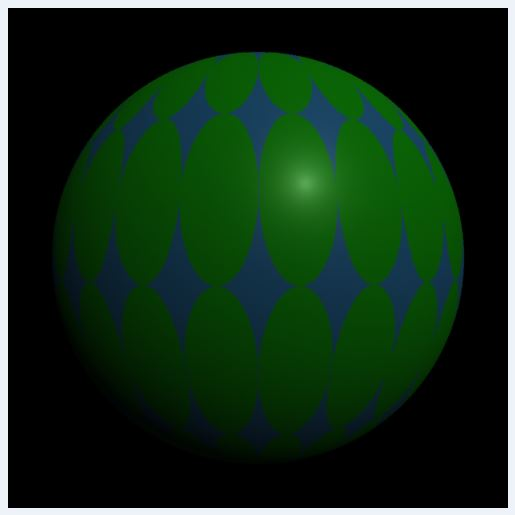
\includegraphics[width=2.9in]{surface_mag_00.jpg}
\end{center}
Then the noise is added into the surface shader. By following the noise equation on the class note: $N = NoiseMag * noise( NoiseFreq * PP )$ the noise will be created. In the equation, $PP$ is the coordinate we are working on, and the $noise()$ function messes up the coordinate based on the $NoiseFreq$, which will result to some other points that close to the $PP$ coordinate. This will make the ``noised'' pattern continually. Then by multiply the result with a coefficient, the noise will become different. The following two images show the result images for setting coefficient to $0.1$ and $0.3$.
\begin{center}
	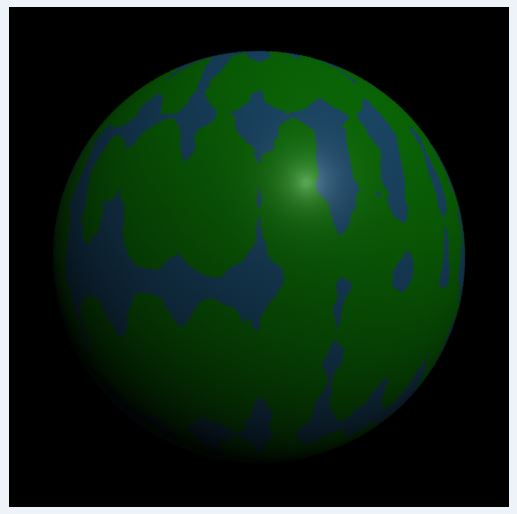
\includegraphics[width=3in]{surface_mag_01.jpg}
	\includegraphics*[width=3in]{surface_mag_03.jpg}
\end{center}
The displacement shader has nothing to do with the colors on the shpere surface. It makes the shpere surface ``pop out'' or ``sink in'' and recalculate the surface normal at the same time. In this project, I only implement the displacement shader ``pop out'' from the surface. Based on the ellipse equation, for one ellipse, the distances to the center point are $1$ on the edge and $0$ at the center. However, if I want to implement ellipses ``pop out'', the displacements should be $0$ on the edge and $1$ at the center. The simplest way to achieve it will be using $1 - distance$ to implement the displacement. However, this will cause the ``sharp'' edges around the ellipses like the left image shown below. So I used a ``\textit{smoothstep}'' function to let the edges also smooth. The result without noise is in the right image listed below.
\begin{center}
	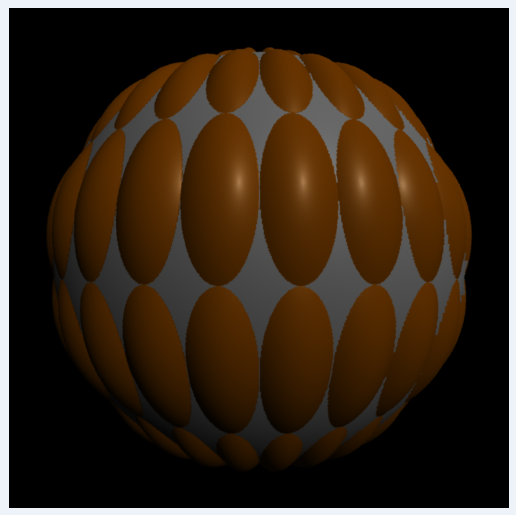
\includegraphics[width=3in]{disp_mag_0.png}
	\includegraphics*[width=3in]{disp_mag_00.jpg}
\end{center}
Similar to the surface shader, adding noise to the displacement shader could be done in the same way. This time, the actual displacement will be made to the sphere surface with noise, and base on that, the normal of the surface will be recalculated. By using the same parameters as we used in the surface shader, the result will turn out that the noised displacement fits the noised surface pattern. The images below show the results with coefficient setting to $0.1$ and $0.3$.
\begin{center}
	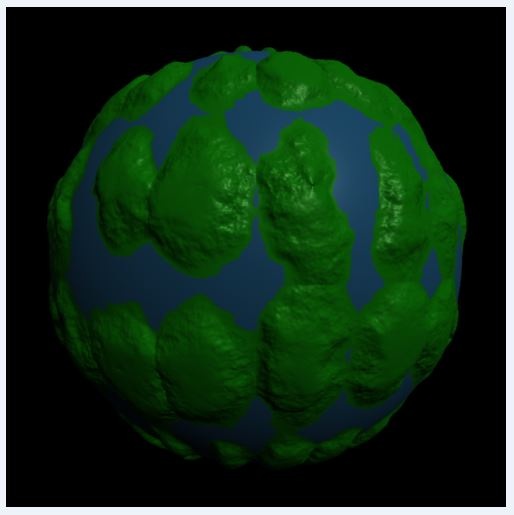
\includegraphics[width=3in]{disp_mag_01.jpg}
	\includegraphics*[width=3in]{disp_mag_03.jpg}
\end{center}
The bump-mapping displacement is not a real displacement. It has a little bit difference in implementing compare to the real displacement. It could be told from the difference in the code. in the noised.sl:
\\
\begin{lstlisting}
if( disp != 0. )
{
	normal n = normalize(N);
	P = P + disp * n;
	N = calculatenormal(P);
}
\end{lstlisting}
The real displacement changes the P value with noised displacement, and then recalculate the normal of the surface. However, in the noiseb.sl:
\\
\begin{lstlisting}
if( disp != 0. )
{
	normal n = normalize(N);
	N = calculatenormal( P + disp * n );
}
\end{lstlisting}
The bump-mapping doesn't change the P value, but just use it to recalculate the normal. Under this case, there is no real displacement made to the surface. The reason why the bump-mapping doesn't work well in stereo displays is also because of this, the scene could be really awful seen from another direction since there is no real displacement. The result image for bump-mapping is shown in the image below.
\begin{center}
	\includegraphics*[width=3.2in]{bump_mag_03.jpg}
\end{center}
\section{Summary}
This project is a little bit harder than the last project and I did meet some problems during the process. For example I forgot adding ``Attribute'' to the ``.rib'' file and the whole sphere turned out really ugly, I used different coefficients for surface and displacement shaders so their results didn't match, and I passed wrong value to ``old radius'' so that my ellipses all became donuts when I applied noise on them. However, solving these problems let me learned a lot more about shaders and had a deeper understanding for what really going on in the code. The final result I had are also pretty fun to play with. I hope I could learn more about this in the following classes.
\end{document}